\beginSupplementaryMaterials

%%%%%%%%%%%%%%%%%%%%%%%%%%%%%%%%%%%%%%%%%%%%%%%%%%%%%%%%%%%%%%%%%%%%%%%%%%%%%%%%%%%%%%%%%%%%%%%%%%%%%%%%%%%%%%
\section{Algorithm Details}
\label{app:fb_algo_details}
Following prior work on Forward-Backward (FB) representations \citep{touati2023does}, we include two additional regularization losses to stabilize FB training. First, we adopt an orthonormality regularization on the backward representation $
\Sigma_B = \mathbb{E}\left[B(s)B(s)^\top\right]$,
which encourages the covariance of $B(s)$ to approach the identity matrix. This regularization prevents the backward representation from collapsing and improves the conditioning of the learned embedding space. Second, we introduce a temporal-difference regularization loss on the forward map that encourages $
F(s,a,z)^\top z
$ to approximate the action-value function corresponding to the reward induced by $B(s)^\top \Sigma_B^{-1}z$. This loss encourages the forward representation to capture directions in the latent space that are relevant for policy optimization. See \citep{touati2023does} (Appendix B) for more details.

%%%%%%%%%%%%%%%%%%%%%%%%%%%%%%%%%%%%%%%%%%%%%%%%%%%%%%%%%%%%%%%%%%%%%%%%%%%%%%%%%%%%%%%%%%%%%%%%%%%%%%%%%%%%%%

% \section{Prior Information on Rewards}
% \todo{unfinished}
% $\phi(s,a) = [v, \omega,g,h]$ where $v$ is the 3-dimension base linear velocity, $\omega$ is the 3-dimension base angular velocity, $g$ is the 3-dimension base gravity vector and h is 1-dimension base height. 

%%%%%%%%%%%%%%%%%%%%%%%%%%%%%%%%%%%%%%%%%%%%%%%%%%%%%%%%%%%%%%%%%%%%%%%%%%%%%%%%%%%%%%%%%%%%%%%%%%%%%%%%%%%%%%
\section{Practical Exploration}
\label{appendix:practical-exploration}
To improve exploration efficiency in this setting, we discard states where the robot pitch or roll exceeds $21.5^\circ$. These states typically correspond to failure events such as falling, which can produce large velocities unrelated to meaningful locomotion behaviors. Filtering such degenerate transitions helps focus exploration on valid locomotion regimes.
%%%%%%%%%%%%%%%%%%%%%%%%%%%%%%%%%%%%%%%%%%%%%%%%%%%%%%%%%%%%%%%%%%%%%%%%%%%%%%%%%%%%%%%%%%%%%%%%%%%%%%%%%%%%%%

\section{Ablation Tests}
\subsection{Ablation Study on $\beta$.} 
\label{appendix:ablation_beta}
\Cref{fig:Abalation} presents the ablation results with different inverse-density coefficients $\beta$. When $\beta=0$, corresponding to uniform latent sampling without density reweighting, both entropy and task reward remain relatively low. As $\beta$ increases, entropy and reward consistently improve.

These results confirm that inverse-density reweighting effectively increases the entropy of the achieved behavior distribution and mitigates replay buffer occupancy collapse during online training.

% \begin{figure}[H]
%     \centering
%     \includegraphics[width=0.6\linewidth]{figure/experiments_ablation_2.png}
%     \caption{Comparison between different betas}
%     \label{fig:placeholder}
% \end{figure}

\begin{figure}[H]
    \centering
    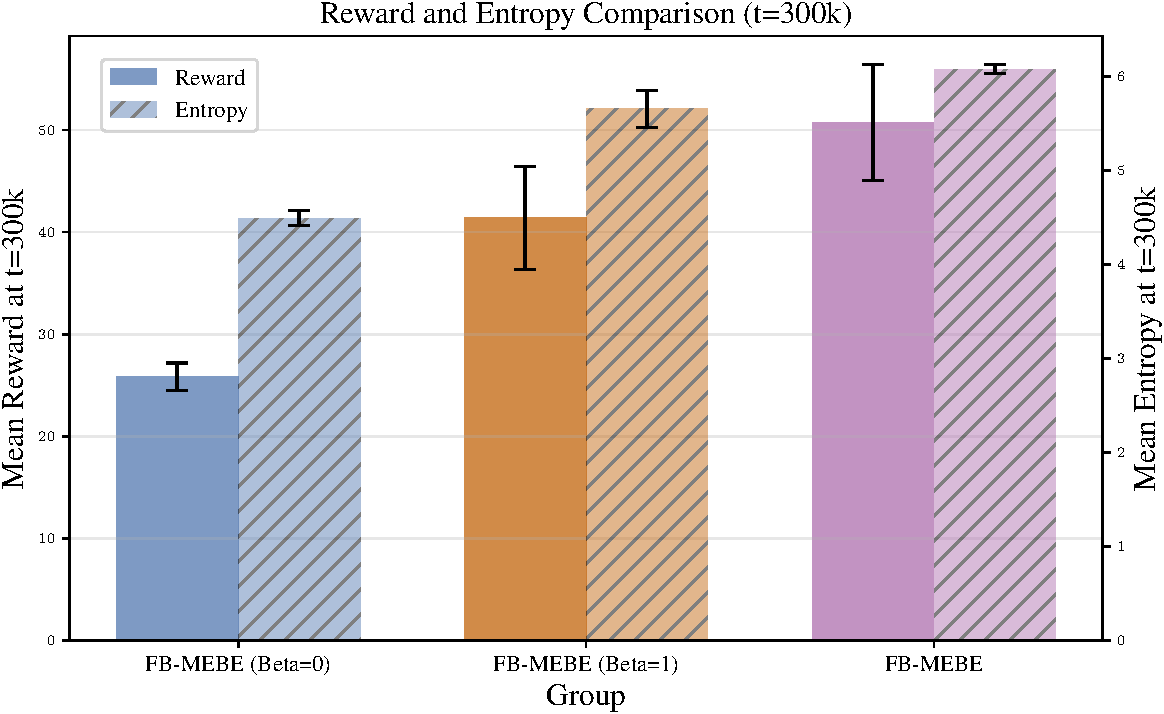
\includegraphics[width=0.6\linewidth]{figure/fb-mebe-comparison-beta.pdf}
    \caption{Comparison between different betas on FB-MEBE on locomotion tasks}
    \label{fig:Abalation}
\end{figure}
\subsection{Ablation study on sampling strategy}
\label{appendix:ablation_exptrain}
We evaluate a version of \method (\method-\text{abl}), that performs an ablation on the sampling strategy used for \textit{training} the FB representations.
\method uses the \textit{same} sampling strategy for reward embeddings used for data collection ($0.8 z_{exp}$ + $0.2 z_{random}$) and the reward embedding used for training FB representations.
Here, we compare with an alternative version which only uses our  strategy for data collection, and uses $(0.8 z_\text{goal reaching} + 0.2 z_\text{random}$ for training. The later is analogous to the exploration strategy $\method(\beta=0)$ uses.
While \method puts more emphasis on learning FB representations and policies for low visitation behaviors and might hence learn better policies useful for exploration,\method-\text{abl} samples exploration behaviors uniformly from the replay buffer.
While these two approaches are different in nature, in practice we do not find significant differences as can be seen in \Cref{fig:ablation_exptrain1}. Extensive evaluation on different mixing ratios can also bring more insights on better sampling alternatives.


% TEMP
\begin{figure}
    \centering
    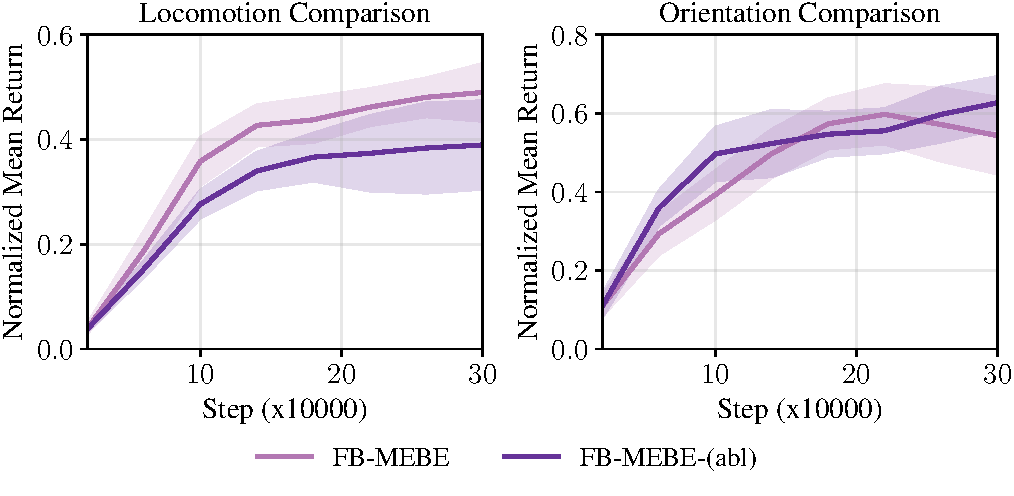
\includegraphics[width=0.8\linewidth]{figure/compare_exp_with_exp_and_train.pdf}
    \caption{Comparison on velocity-tracking tasks between \method and an ablation \method-\text{abl} leveraging different sampling strategies for training the FB algorithm}
    \label{fig:ablation_exptrain1}
\end{figure}


%%%%%%%%%%%%%%%%%%%%%%%%%%%%%%%%%%%%%%%%%%%%%%%%%%%%%%%%%%%%%%%%%%%%%%%%%%%%%%%%%%%%%%%%%%%%%%%%%%%%%%%%%%%%%%
\section{Replay buffer data distribution}
\label{appendix:replay_buffer_data_distribution}
\begin{figure}[H]
    \centering
    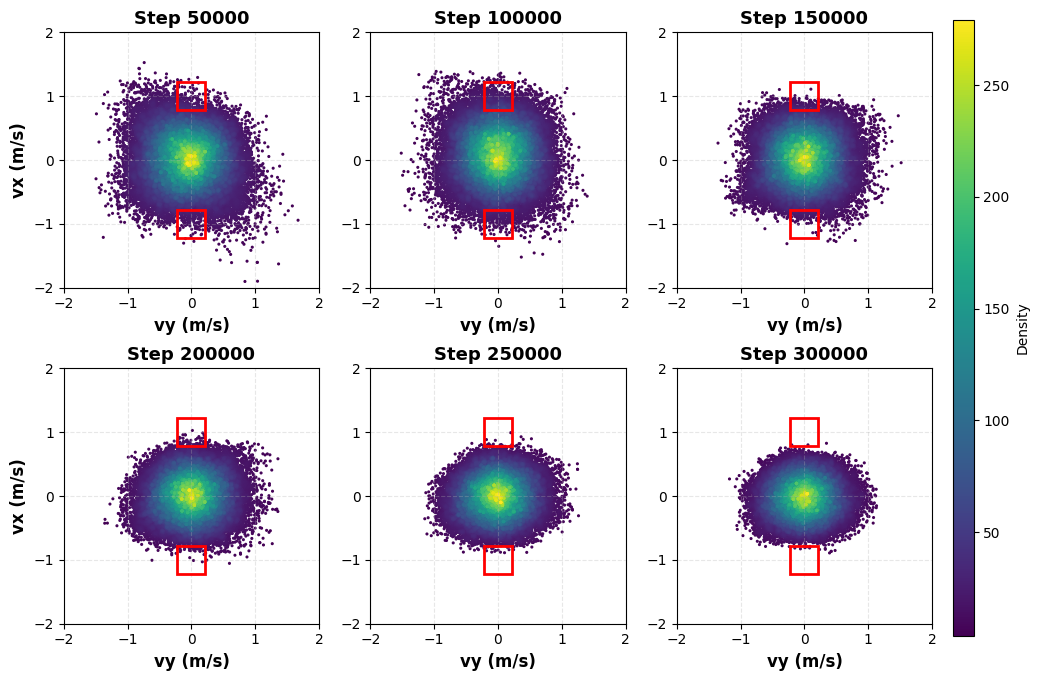
\includegraphics[width=0.8\linewidth]{figure/Appendix_FB_buffer_change.png}
    \caption{Velocity $\left[v_x, v_y \right]$ distribution of FB replay buffer at different training step. The color represents the density of data points.}
    \label{fig:replay_buffer_data_distribution}
\end{figure}


%%%%%%%%%%%%%%%%%%%%%%%%%%%%%%%%%%%%%%%%%%%%%%%%%%%%%%%%%%%%%%%%%%%%%%%%%%%%%%%%%%%%%%%%%%%%%%%%%%%%%%%%%%%%%%
\section{Task Reward Function}
\label{appendix:reward-function}

 Let $\mathbf{v} \in \mathbb{R}^3$ and $\boldsymbol{\omega}_z \in \mathbb{R}$ denote the current base linear velocity and yaw angular velocity, respectively,  $h \in \mathbb{R}$ denote the current base height and let $\mathbf{g} \in \mathbb{R}^3$ denote the projected gravity vector. The corresponding command targets are denoted by $\mathbf{v}^\ast$, $\omega_z^\ast$,  $h^*$, and $\mathbf{g}^\ast$.\\
\\
We define the tracking errors as
\begin{align}
e_v &= \lVert \mathbf{v} - \mathbf{v}^\ast \rVert_2, \\
e_\omega &= \lvert \omega_z - \omega_z^\ast \rvert, \\
e_g &= \lVert \mathbf{g} - \mathbf{g}^\ast \rVert_2 \\
e_h &=  \lVert h - h^\ast \rVert_2.
\end{align}
\\
The individual reward terms are computed using Gaussian-shaped functions:
\begin{align}
r_v &= \exp\left(-\left(\frac{e_v}{0.3}\right)^2\right), \\
r_\omega &= \exp\left(-\left(\frac{e_\omega}{0.2}\right)^2\right), \\
r_g &= \exp\left(-\left(\frac{e_g}{0.1}\right)^2\right), \\
r_h &= \exp\left(-\left(\frac{e_h}{0.05}\right)^2\right).
\end{align}
\\

The locomotion and orientation task reward is defined as follows:

\begin{align}
r_{\text{locomotion}} &= r_v \cdot r_\omega \cdot r_g \\
r_{\text{orientation}} &= r_g \cdot r_h
\end{align}

The reward for sim-to-real transfer is defined by multiplication of all terms:
\begin{equation}
r_{\text{sim2real}} = r_v \cdot r_\omega \cdot r_g \cdot r_h
\end{equation}

%%%%%%%%%%%%%%%%%%%%%%%%%%%%%%%%%%%%%%%%%%%%%%%%%%%%%%%%%%%%%%%%%%%%%%%%%%%%%%%%%%%%%%%%%%%%%%%%%%%%%%%%%%%%%%
\section{Regularization rewards}
\label{appendix:regularization_reward}

We provide the mathematical definitions of the regularization reward.  Let $N_j$ denote the number of actuated joints and $N_f$ the number of feet. At time step $t$, let $\ddot{\mathbf{q}}_t \in \mathbb{R}^{N_j}$ be the joint acceleration vector, $\mathbf{a}_t \in \mathbb{R}^{N_j}$ be the action vector, and $\mathbf{a}_{t-1}$ be the previous action.  For each foot $i \in \{1,\dots,N_f\}$, let $h_{t,i}$ be its vertical position (world frame), and $\mathbf{v}^{xy}_{i,t} \in \mathbb{R}^{2}$ be its horizontal linear velocity (world frame). \\

\paragraph{Joint acceleration penalty.}
The joint-acceleration penalty is defined as the squared $\ell_2$ norm of the joint acceleration vector:
\begin{equation}
r_{\text{joint\_acc}}
=
\|\ddot{\mathbf{q}}_t\|_2^2
=
\sum_{k=1}^{N_j} \left(\ddot{q}_{t,k}\right)^2 .
\end{equation}

\paragraph{Action rate penalty.}
The action-rate penalty discourages abrupt changes between consecutive actions:
\begin{equation}
r_{\text{action\_rate}}
=
\|\mathbf{a}_t - \mathbf{a}_{t-1}\|_2^2
=
\sum_{k=1}^{N_j} \left(a_{t,k}-a_{t-1,k}\right)^2 .
\end{equation}

\paragraph{Feet slippage.}
The feet-slide penalty penalizes horizontal foot motion during ground contact.
A binary contact indicator $c_{t,i}$ is defined as
\begin{equation}
c_{t,i}
=
\begin{cases}
1, & \text{if } h_{t,i} > h_{\mathrm{feet\_contact}}, \\
0, & \text{otherwise}.
\end{cases}
\end{equation}

\begin{equation}
r_{\mathrm{feet\_slide}}
=
\sum_{i=1}^{N_f}
c_{t,i}
\,
\|\mathbf{v}_{t,i}^{xy}\|_2 .
\end{equation}

% \paragraph{Feet air-time reward.}
% Let $c_{i,t}\in\{0,1\}$ be an indicator of \emph{first contact} for foot $i$ at step $t$ (i.e., $c_{i,t}=1$ iff the foot transitions from air to contact),
% and let $T^{\text{air}}_{i,t}\ge 0$ be the \emph{last air time} accumulated for foot $i$ before this contact.
% Given a threshold $\tau = 0.5$, the air-time reward is:
% \begin{equation}
% r_{\text{air}} \;=\; \sum_{i=1}^{N_f} \left(T^{\text{air}}_{i,t}-\tau\right)\, c_{i,t}.
% \end{equation}

% \paragraph{Feet clearance reward.}
% Given a target clearance height $h^\star = 0.1$, a scale parameter $\sigma = 0.005$ (named \texttt{std} in code),
% and $\kappa = 2.0$ (named \texttt{tanh\_mult}), we define for each foot:
% \begin{equation}
% e_{i,t}
% \;=\;
% \left(h_{i,t}-h^\star\right)^2
% \;\cdot\;
% \tanh\!\Big(\kappa \, \left\|\mathbf{v}^{xy}_{i,t}\right\|_2\Big),
% % \end{equation}
% and the clearance reward is computed as:
% \begin{equation}
% r_{\text{clearance}}
% \;=\;
% \exp\!\left(
% -\frac{\sum_{i=1}^{N_f} e_{i,t}}{\sigma}
% \right).
% \end{equation}

\paragraph{Total typical regularization reward.}
In our experiments, the regularization reward used to train the critic is:
\begin{equation}
r_{\text{reg}} =
-2.5\times 10^{-7}\, r_{\text{joint\_acc}}
-0.1\, r_{\text{action\_rate}}
-0.1\, r_{\text{feet\_slide}}
\end{equation}


\section{Regularized Exploration.}
\label{appendix:qregu}
We use critic $Q_{\text{reg}}(s,a)$ to estimate the long-term return of the barrier regularization reward $r_{\text{reg}}$ defined in \Cref{appendix:regularization_reward}. Given tuples $(s,a,r_{\text{reg}},s')$ sampled from the replay buffer, we train the regularization critic by minimizing a standard temporal-difference (TD) loss:
\begin{equation}
\mathcal{L}_{\text{critic}}(Q_\text{reg})
=
\mathbb{E}_{ (s,a,s')\sim \rho,a'\sim\pi_z (s')}\Big[
\big(
Q_{\text{reg}}(s,a)
-
\big(r_{\text{reg}}
+
\gamma \,
\bar Q_{\text{reg}}(s', a')
\big)
\big)^2
\Big]
\label{eq:reg_critic_loss}
\end{equation}
\\
Therefore, to pretrain FB agent and learn good gait at the same time, we have the following actor loss:
\begin{equation}
\mathcal{L}_{\text{actor}}(\pi)
=
-\mathbb{E}_{z\sim\nu,\; s\sim\rho,\; a\sim\pi_z(s)}\Big[
Q_{\text{FB}}(s,a,z)
+
\lambda_{\text{reg}}\,
Q_{\text{reg}}(s,a)
\Big]
% \label{eq:actor_loss_with_reg}
\end{equation}

%%%%%%%%%%%%%%%%%%%%%%%%%%%%%%%%%%%%%%%%%%%%%%%%%%%%%%%%%%%%%%%%%%%%%%%%%%%%%%
\newpage % split page temporarily (will delete later)
\section{Simulation Setup}

\paragraph{Joint Control}
We employ joint position control as the low-level control interface. The joint configuration of the robot in the standing pose is defined as the nominal joint position $q_{nom}$. The policy outputs joint position offsets $a$, which are scaled by a factor $s$ and added to the nominal configuration to obtain the target joint positions
\begin{equation}
q_{target} = q_{nom} + s \cdot a .
\end{equation}
The target joint positions are tracked using a PD controller
\begin{equation}
\tau = K_p (q_{target} - q) + K_d (\dot{q}_{target} - \dot{q}),
\end{equation}
where $q$ and $\dot q$ denote the current joint positions and velocities.

\begin{table}[H]
\centering

\begin{minipage}[t]{0.48\textwidth}
\centering
\caption{Joint Control Parameters}
\vspace{0pt}
\begin{tabular}{l c}
\toprule
\textbf{Parameter} & \textbf{Value} \\
\midrule
Action Scale 
    & $0.5$ \\
Proportional Gain $K_p$ 
    & $25.0$\\
Derivative Gain $K_d$ 
    & $0.5$\\
Control Frequency [Hz] 
    & $50\text{Hz}$\\
\bottomrule
\end{tabular}

\end{minipage}
\end{table}

\paragraph{Domain Randomization and Observation Noise}
\begin{table}[H]
\centering

\begin{minipage}[t]{0.48\textwidth}
\centering
\caption{Domain Randomization}
\vspace{0pt}
\begin{tabular}{l c}
\toprule
\textbf{Parameter} & \textbf{Range} \\
\midrule
Friction Coefficient 
    & $\mathcal{U}([0.5,\,1.5])$ \\
Base COM Offset [m] 
    & $\mathcal{U}([-0.05,\,0.05])$ \\
Base Mass perturbation [kg]
    & $\mathcal{U}([-2.0,\,2.0])$ \\
Link Mass Offset [m] 
    & $\mathcal{U}([-0.01,\,0.01])$ \\
Link Mass perturbation [kg]
    & $\mathcal{U}([-0.2,\,0.2])$ \\
Default Joint Pos [rad] 
    & $\mathcal{U}([-0.3,\,0.3])$ \\
\bottomrule
\end{tabular}
\end{minipage}
\hfill
\begin{minipage}[t]{0.48\textwidth}
\centering
\caption{Additive Observation Noise}
\vspace{0pt}
\begin{tabular}{l c}
\toprule
\textbf{Observation} & \textbf{Range} \\
\midrule
$v$ [m/s] 
    & $\mathcal{U}([-0.1,\,0.1])$ \\
$\omega$ [rad/s] 
    & $\mathcal{U}([-0.2,\,0.2])$ \\
$\mathrm{grav}$ 
    & $\mathcal{U}([-0.05,\,0.05])$ \\
$q$ [rad] 
    & $\mathcal{U}([-0.01,\,0.01])$ \\
$\dot{q}$ [rad/s] 
    & $\mathcal{U}([-0.15,\,0.15])$ \\
\bottomrule
\end{tabular}
\end{minipage}

\end{table}

%%%%%%%%%%%%%%%%%%%%%%%%%%%%%%%%%%%%%%%%%%%%%%%%%%%%%%%%%%%%%%%


\section{Observation Space}
\label{appendix:observation-space}
\begin{table}[H]
  \centering
  \renewcommand{\arraystretch}{1.15}
  \begin{tabular}{l l}
    \toprule
    Network & Obs Dimension Breakdown\\
    \midrule

    Critic $(F)$ 
    & $ \left[ \mathbf{v}_{3}, \boldsymbol{\omega}_{3}, \mathbf{g}_{3}, h_{\text{base},1}, \mathbf{q}_{12}, \dot{\mathbf{q}}_{12} \right]$ \\

    $B$ 
    & $ \left[ \mathbf{v}_{3}, \boldsymbol{\omega}_{3}, \mathbf{g}_{3}, h_{\text{base},1} \right]$ \\

    Actor
    & $ \left[ \mathbf{v}_{3}, \boldsymbol{\omega}_{3}, \mathbf{g}_{3}, \mathbf{q}_{12}, \dot{\mathbf{q}}_{12}, \mathbf{a}_{12} \right]$ \\

    Critic (Reg)
    & $\left[ \mathbf{v}_{3}, \boldsymbol{\omega}_{3}, \mathbf{g}_{3}, h_{\text{base},1}, \mathbf{q}_{12}, \dot{\mathbf{q}}_{12}, \mathbf{a}_{12}, h_{\text{feet},4}, F_{\text{feet},4} \right]$ \\

    \bottomrule
  \end{tabular}

  \caption{Inputs for different networks}
  \label{tab:fb_inputs}
\end{table}

    \footnotesize
    \begin{flushleft}
    The subscripts represent the dimension of this variable. $\mathbf{v}$ is the base linear velocity, $\boldsymbol{\omega}$ is the base angular velocity, $\mathbf{g}$ is the projected gravity vector, $h_{\text{base}}$ is the base height, $\mathbf{q}$ and $\dot{\mathbf{q}}$ are joint positions and joint velocities, respectively, $\mathbf{a}$ is the last action, $h_{\text{foot}}$ denotes foot heights (4 feet), and $F_{\text{feet}}$ denotes foot contact forces (4 feet). $^{*}$.
    \end{flushleft}
    \normalsize

\textbf{Note on B mapping}: We note that the B representation acts on a lower-dimensional projection of the full state space instead.  When dealing with high dimensionality environments, learning future probabilities for all states is difficult and generally requires large $d$ to accommodate for all possible rewards.
In general, we are often interested in rewards that depend not on the full state but on a projection of it.
If this is known in advance, the representation B can be trained on that part of the state only, with same theoretical guarantees (Appendix, Theorem 4 \citep{touati2021learning}). Hence, we leverage an environment-dependent feature map $\vartheta: S \rightarrow G$, and learn $B(g)$ instead of $B(s)$, where $g=\vartheta(s)$.
Importantly, rewards can be arbitrary functions of g. This was also suggested in \citep{touati2021learning}.


%%%%%%%%%%%%%%%%%%%%%%%%%%%%%%%%%%%%%%%%%%%%%%%%%%%%%%
% \newpage % split page temporarily (will be deleted later)
\section{Hyper-parameters}
\label{appendix:hyperparams}

\begin{table}[H]
\centering
\small
\setlength{\tabcolsep}{12pt}
\renewcommand{\arraystretch}{1.15}
\begin{tabular}{l r}
\toprule
\textbf{Hyperparameter} & \textbf{Value} \\
\midrule
Number of training steps& 150k\\
Number of parallel environments & 2048\\
Number of rollout steps between each agent update & 10\\
Number of gradient steps per agent update & 10\\
Policy delay (TD3 actor update interval) & 2 \\
Number of initial steps with random actions & 1000\\
 Number of samples for task inference&100k\\
Replay buffer size & 4M\\
Batch size & 4096\\
Discount factor & 0.98 \\
 $z$ update step interval&100\\
 $z$ dimension $d$&50\\
 $z$ distribution $\nu$&\\
 ~~ -uniform on unit sphere&20\%\\
 ~~ -goals from online buffer&80\%\\
 Coefficient for orthonormality loss&100\\
 Coefficient for Fz-regularization loss&0.1\\
 Regularization coefficient $\lambda_\text{reg}$&20\\
\bottomrule
\end{tabular}
\caption{Training hyperparameters}
\label{tab:train_hparams}
\end{table}





\label{appendix:fb_hparams}
\begin{table}[H]
\centering
\small
\setlength{\tabcolsep}{10pt}
\renewcommand{\arraystretch}{1.15}
\begin{tabular}{lcccc}
\toprule
\textbf{Hyperparameter} &
\textbf{Critic $(F)$} &
\textbf{B} &
\textbf{Critic $(\text{Reg})$} &
\textbf{Actor} \\
\midrule
Learning Rate &
$5\cdot 10^{-5}$ &
$5\cdot 10^{-5}$ &
$5\cdot 10^{-5}$ &
$5\cdot 10^{-5}$ \\

Soft update coefficient& 
$0.01$& 
$0.01$& 
$0.005$&
$0.01$\\

Input Variables &
$(s, a, z)$ &
$(s)$ &
$(s, a)$&
$(s, z)$ \\

Output Dim &
$d$ &
$d$ &
$1$ &
$12$ \\

Embedding Hidden Units &
$1024$ &
-- &
--&
$1024$ \\

Feed Forward Hidden Layers &
$2$ &
$2$ &
$4$&
$2$ \\

Feed Forward Hidden Units &
$1024$ &
$512$ &
$1024$ &
$1024$ \\

Activations &
ReLU &
ReLU &
ReLU &
ReLU \\

Number of Parallel Networks &
$2$ &
$1$ &
$2$ &
$1$ \\
\bottomrule
\end{tabular}
\caption{Network hyperparameters}
\label{tab:fb_hparams}
\end{table}

\paragraph{Normalizing Flow and Reverse Sampling}

\begin{table}[H]
\centering
\caption{Hyperparameters of the Normalizing Flow.}
\begin{tabular}{l c}
\toprule
\textbf{Hyperparameter} & \textbf{Value} \\
\midrule
Flow architecture & RealNVP-style normalizing flow \\
Number of coupling layers & 10 \\
Hidden dimension & 64 \\
Activation function & ReLU \\
Scale output activation & Tanh \\
Masking strategy & Alternating checkerboard / channel mask \\
Base distribution & Standard Gaussian $\mathcal{N}(0, I)$ \\
Learning rate & $1\cdot 10^{-3}$ \\
Batch size & 256 \\
Training epochs & 30 \\
Goal buffer size & 10k \\
\bottomrule
\end{tabular}
\label{tab:nf_hyperparameters}
\end{table}

\begin{table}[H]
\centering
\caption{Hyperparameters of reverse sampling.}
\begin{tabular}{l c}
\toprule
\textbf{Hyperparameter} & \textbf{Value} \\
\midrule
normallizing flow update frequency & 1000 steps \\
sample buffer size & 100k \\
$\epsilon$ (for stability) & 0.1 \\
$\beta$ (reverse sampling strength) & 2.0 \\
\bottomrule
\end{tabular}
\label{tab:reverse_sampling_hyperparameters}
\end{table}

%%%%%%%%%%%%%%%%%%%%%%%%%%%%%%%%%%%%%%%%%%%%%%%%%%%%%%%%%%%%%%%%%%%%%%%%%%%%%%%%%%%%%%%%%%%%%%%%%%%%%%%%%%%%%%

\section{Connection to Universal Successor Features}
\label{appendix:extended_rel_work}
Given a feature map $\phi: \gS \rightarrow \sR^d$ that embeds states into d-dimensional features,  the successor features \citep{barreto2017successor} for policy $\pi$ are defined as $\Phi^\pi(s,a) = \mathbb{E}\big[\sum_{t\geq0}\gamma^t \phi(s_{t+1}) | s,a,\pi\big]$. Then for any reward function that can be expressed as a linear combination of the features, i.e., $r(s)= z^\top\phi(s)$, where $z \in \sR^d$ are the weights, the Q-function can be expressed as: $Q_r^\pi(s,a) = z^\top\Phi^\pi(s,a)$. 
Universal successor features (USF) \citep{borsauniversal}, goes one step further and allows not only zero-shot policy evaluation, but a generic framework for zero-shot policy optimization. This is achieved by learning a family of policies $\{\pi_z\}$ parameterized by a latent vector $z \in \sR^d$, such that for each $z$, the policy $\pi_z$ is trained to be optimal with respect to reward function $r_z:= z^\top\phi$. Formally,
\begin{equation}\label{eq:usf}
   \mathbb{E}\Big[\sum_{t\geq0}\gamma^t \phi(s_{t+1}) | s,a,\pi\Big], \quad \pi_z(s) = \argmax_{a} \Phi(s,a,z)^\top  z.
\end{equation}
There exist several instantiations of USF \citep{agarwal2024proto, park2024foundation} (see \citep{touati2023does} for an extensive list), however, they requires a separate methods for learning features $\phi$ and one for learning its successor features, usually via a TD-learning approach. In contrast, the forward backward representation \citep{touati2021learning} provides an alternative framework for zero-shot RL that jointly learns the features and its successor features, via a contrastive learning approach. 

FB representations are closely related to successor features. In fact, $F(s,a,z)$ is the successor feature of policy $\pi_z$ of the basic features $\phi(s)= \text{Cov}_{\rho}(B)^{-1}B(s)$ \citep{touati2023does}, where $\text{Cov}_{\rho}B=\mathbb{E}_{\tilde s\sim\rho}\big[B(\tilde s)B(\tilde s)^\top \big]$.

After training, given a reward function $r$ specified at test time, we can find the task embedding $z_r$ parameterizing the optimal learnt policy for reward $r$, by performing a simple linear regression of $r$ onto the span of the learnt features $B$. Namely we find the weights $z_r^*$ (coordinates of the feature basis) that minimize $z_r^* = \argmin_z \mathbb E_{s\sim\rho}\big[ \big((r(s) - z_r^\top \phi(s)\big)^2] = \text{Cov}_{\rho}(\phi)^{-1} \mathbb{E}_{\tilde s\sim\rho}\big[\phi(s)r(s)\big]$. 
For FB, the reward embedding can be computed simply via $z_r = \mathbb{E}_{s\sim\rho}\big[B(s)r(s)\big]$ \citep{touati2021learning}, where the expectation is approximated through sampling from the dataset distribution used for training (or a subset).